We performed resolution tests for models with [Fe/H] $\in \{-1.2, -0.4, 0.4\}$ and $M \in \{0.9, 1.3, 1.7\}$ using the Brown thermohaline mixing prescription.
We studied a grid of \texttt{mesh\_delta\_coeff} and \texttt{time\_delta\_coeff} values which span from 0.1 to 1.0 over five log-space steps.
We measure $r$ in each of these models, and in Fig.~\ref{Fig:resolution_test} we plot the absolute value of the relative error between that $r$ value and the reference $r_{\rm ref}$ value reported for that case in Fig.~\ref{fig:mesa_r_spread}.
We calculate the relative error to be $1 - r/r_{\rm{ref}}$.

We find that small values of the mesh coefficient combined with large values of the time coefficient result in large errors.
This occurs because the front of the thermohaline zone, and sometimes the full thermohaline zone, becomes numerically unstable, and large oscillations in $R_0$ lead to large errors in the $r$ calculation.
Furthermore, we find that when the thermohaline front is not properly numerically resolved, it does not propagate upwards in mass coordinate and connect with the convective shell.


\begin{figure*}[!tb]
\begin{center}
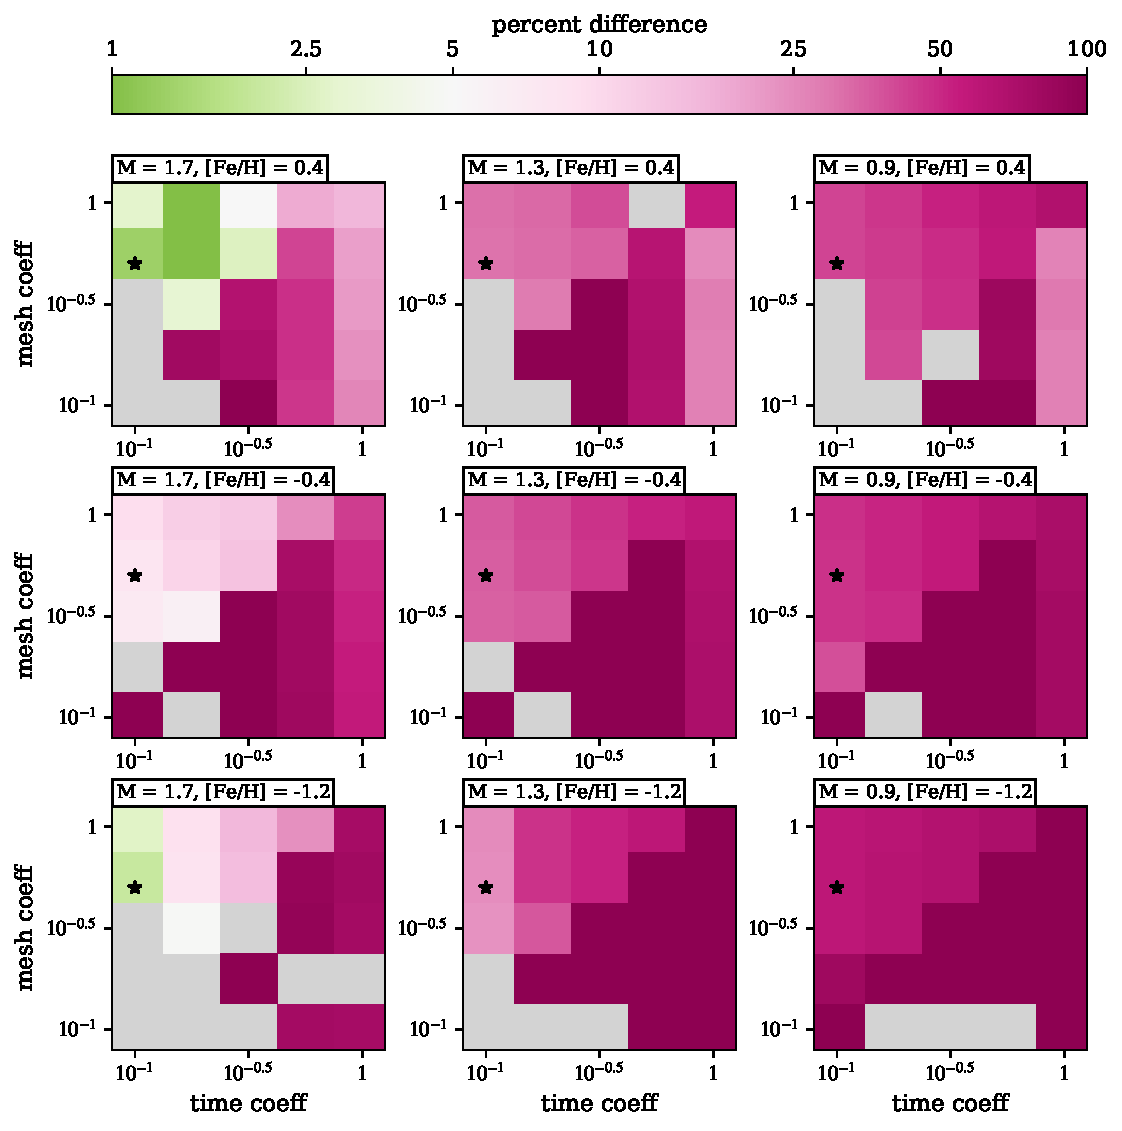
\includegraphics[width=\textwidth]{resolution_test.pdf}
\caption{This is a template figure showing relative error in a calculation as a function of mesh and time delta coefficient. It'll look nicer. It also won't have the same data repeated 9 times once the data finish running!}
\label{Fig:resolution_test}
\end{center}
\end{figure*}